% Preambulo
\documentclass[10pt,letterpaper,twocolumn]{article}
\usepackage[spanish,es-tabla]{babel} % idioma: Español, no coloque nombre tablas como cuadro
\usepackage[T1]{fontenc} \usepackage[utf8]{inputenc} % símbolos especiales del idioma
\usepackage{times}
\usepackage[calc,showdow,spanish]{datetime2}
\parindent = 0cm % configuración de sangría
\usepackage[backend=biber,style=ieee]{biblatex}
\usepackage{tabularx} % extra features for tabular environment
%\usepackage{amsmath} \usepackage{amssymb,amsfonts,latexsym,cancel}  % símbolos matemáticos 
\usepackage{array}
%\usepackage{bm}
%\usepackage{epstopdf} % figuras en formato eps a pdf
\usepackage{hyperref} % agregar hiper enlaces dentro del archivo PDF generado
\usepackage{longtable} % habilitar tablas largas
%\setcounter{MaxMatrixCols}{40} % configuración de limite columnas: 40
%\usepackage{multicol} % varias columnas al documento
\usepackage{subfigure} % varias figuras
\usepackage[small,compact]{titlesec} \usepackage{titling} %cambiar el formato del titulo
%\newcolumntype{E}{>{$}c<{$}} % información de tablas en formato matemático
\usepackage{graphicx} % takes care of graphic including machinery
\usepackage{geometry} % configuración del dimensiones de la margen del documento 
\usepackage{booktabs}
%\usepackage{subcaption}
\usepackage{tcolorbox}
\usepackage{fancyhdr} % configuración del formato del documento
\usepackage{authblk}
\usepackage[font=footnotesize]{caption}
\usepackage[toc,page]{appendix}
\usepackage{parskip}
\usepackage{amssymb, amsmath} % Paquetes matemáticos de la American Mathematical Society
\usepackage{float}
\usepackage{setspace}
\usepackage{parskip}
\usepackage{multirow}
\usepackage[all]{xy}
\usepackage{tikz}
\usepackage{tikz}
\usepackage{circuitikz}
\usetikzlibrary{positioning,circuits.ee.IEC}
\usetikzlibrary{matrix}
\usetikzlibrary{calc}
\usetikzlibrary{fit}
\usepackage{fourier}
\usepackage{makecell,cellspace,caption}
\usepackage{color,colortbl}
\usepackage[first=0,last=9]{lcg}
\usepackage{hhline} 
%\usepackage{showframe}
    
%
%
% Configuración de margen
\geometry{
	papersize = {216mm, 279.4mm},
	width = 18cm,
	height = 25cm,
	headsep = 5mm,
	head = 1cm,
	marginpar = 2mm,
	includeall,
}
%
%
% Configuración de hipervinculos
\hypersetup{
	colorlinks = true, % falso: enlace en caja; verdadero: enlaces de colores
	linkcolor = black, % color de los enlaces internos
	citecolor = blue, % color de los enlaces a la bibliografía
	filecolor = magenta, % color de los enlaces de archivos
	urlcolor = black,
}
%
%
% Configuración de estilo de margen


%
%
% Algunas configuraciones del cuerpo del documento
\renewcommand{\tablename}{Tabla}
\renewcommand{\baselinestretch}{1.0} % Para indicar el tamaño del entrelineado
\setlength{\parskip}{1.5mm} % Modificar espacio entre párrafos
\renewcommand*{\bibfont}{\footnotesize} % Cambiar tamaño bibliografía
%
%
% Configuración de estilo para autores y afiliaciones
\renewcommand*{\Authsep}{, }
\renewcommand*{\Authand}{ y }
\renewcommand*{\Authands}{ y }
\renewcommand*{\Affilfont}{\normalsize}
\setlength{\affilsep}{-2mm} % asignar espacio entre autores y afiliaciones
\renewcommand\Authfont{\fontsize{10}{10}\selectfont} % cambiar tamaño de letra autores
\renewcommand\Affilfont{\fontsize{7}{7}\itshape} % cambiar tamaño de letra afiliaciones de autores
%
%
% Carpeta contenedora de las imágenes
\graphicspath{ {codigofuente/img/} }



%
%
% Título, autores e información afiliada a los autores
\title{
	\fontsize{18}{18}\selectfont
	\textbf{Contaminación plástica masiva en un mega-río de un país en desarrollo: Depósito de sedimentos e ingestión por peces (Prochilodus lineatus)*
		\vspace{-1mm}
	}}
\author[1]{Martín C.M. Blettler}
\author[1]{Nicolás Garello}
\author[2]{Léa Ginon}
\author[1]{Elie Abrial}
\author[1]{Luis A. Espinola}
\author[3]{Karl M. Wantzen}
\vspace{-1mm}
\affil[1]{{\textit{National Institute of Limnology (INALI, UNL-CONICET), Santa Fe, Argentina}}\vspace{-2mm}}
\affil[2]{{\textit{University of Polytech Tours (IMA), 37200, Tours,France}}\vspace{-2mm}}
\affil[3]{{\textit {UNESCO Chair ``River Culture\_ Fleuves et Patrimoine'', Tours University, 37200, Tours, France}}\vspace{-2mm}}
\date{}
%
%
% Vincular archivo de biliogarafias
\bibliography{codigofuente/bibliografia.bib}
%
%
% Cuerpo del documento
\begin{document}
%
%
%
\twocolumn[
	\begin{@twocolumnfalse}
		\maketitle
		\vspace{-5mm}
		\begin{abstract}
			El objetivo de este estudio fue determinar la cantidad, composición y origen de los desechos plásticos en uno de los ríos más grandes de Argentina (América del Sur), centrándose en el impacto de los ríos urbanos, relaciones entre macro, meso y microplásticos, cuestiones sociopolíticas y la ingestión de microplásticos por peces.

			Registramos una gran concentración de detritos macroplásticos de origen doméstico (hasta 5.05 artículos macroplásticos por $m^{2}$) dominados principalmente por bolsas (principalmente polietileno de alta y baja densidad), envoltorios de alimentos (polipropileno y poliestireno), plásticos de espuma (poliestireno expandido) y botellas de bebidas (poliestireno tereftalato de etileno), particularmente aguas abajo de la confluencia con un arroyo urbano. Esta sugerencia señala la inadecuada recolección, procesamiento y disposición final de residuos en la región, lo que lamentablemente recurrente en muchas ciudades del Sur Global y en Argentina en particular.

			Encontramos un promedio de 4654 fragmentos microplásticos $m^{2}$ en los sedimentos costeros del río, que van de 131 a 12687 microplásticos $m^{2}$. A diferencia de otros estudios de países industrializados de Europa y América del Norte, microplásticos secundarios (resultantes de la trituración de partículas más grandes) eran más abundantes que los primarios (microperlas para cosméticos o gránulos para la industria). Esto podría explicarse por las diferencias en los hábitos de consumo y el nivel de industrialización entre sociedades y economías.

			Se registraron partículas microplásticas (en su mayoría fibras) en el tracto digestivo del $100\%$ de las \textit{Prochilodus lineatus} (commercial species).

			Contrariamente a las declaraciones publicadas recientemente por otros investigadores, nuestros resultados sugieren que ni los macroplásticos ni los mesoplásticos servirían como sustitutos de los elementos microplásticos en las encuestas de contaminación, lo que sugiere la necesidad de considerar las tres categorías de tamaño.

			La contaminación plástica masiva encontrada en el río Paraná se debe a una gestión inadecuada de los residuos. Se requieren nuevas acciones para gestionar adecuadamente los residuos desde su inicio hasta su disposición final.
		\end{abstract}

	\end{@twocolumnfalse}
]

\section{Introducción}
    La degradación de las cuencas hidrográficas se ha convertido en uno de los más importantes problemas ambientales, sociales y económicos en todo el mundo. México no es una excepción. Similar a muchas cuencas hidrográficas en todo el país, la cuenca del río Ayaquila presenta una compleja gama de problemas derivados del cambio de uso de la tierra, incendios forestales, erosión del suelo, contaminación, agotamiento de las aguas subterráneas, disminución de los caudales de arroyos y ríos, y el uso ineficiente del agua para el abastecimiento de agua y el riego urbano. Además, cuando se combina con la creciente demanda de agua debido al crecimiento de la población en los centros urbanos y el aumento de la producción agrícola, la necesidad de perforar más profundo para extraer agua subterránea o transportar agua de largas distancias pueden, a su vez, producir conflictos locales y regionales.

    En México, la actual organización de las instituciones responsables de aspectos de la gestión de los recursos hídricos sobre una base sectorial no se corresponde con la naturaleza multifuncional del agua. Además, dad la escala y complejidad de la degradación de las cuencas hidrográficas, los niveles de gobierno federal y estatal a menudo carecen de la capacidad operativa para abordar este tipo de problema ambiental. Aquí es donde los gobiernos municipales pueden jugar un papel protagónico, porque es precisamente a nivel de cuenca donde el gobierno local responde de manera más directa a las demandas e iniciativas locales. Cuando varios gobiernos municipales enfrentan problemas comunes en relación con el manejo de la tierra, debido a la intersección de procesos ecológicos y socioeconómicos dentro de las cuencas hidrográficas que trascienden los límites administrativos, es de fundamental importancia aumentar la capacidad institucional para el manejo de los recursos hídricos a través de arreglos intermunicipales, dentro del marco de gestión integrada de cuencas hidrográficas y/o gestión integrada de recursos hídricos.(3)

    La gestión integrada de los recursos hídricos (IWRM) ha surgido precisamente en respuesta a la observación de que la infraestructura y la gestión de los recursos hídricos se han desarrollado tradicionalmente para casa sector relacionado con el agua (como el riego, el suministro de agua urbana, la industria) de forma independiente, con poca o ninguna coordinación entre los sectores. Por lo tanto, la IWRM se refiere a la necesidad de considerar el agua de una manera más holística, teniendo en cuenta todos los aspectos del desarrollo, la gestión y el uso de los recursos hídricos, y los efectos de estos entre sí, sociales y beneficios ambientales del uso del agua. (4)

    \setlength{\leftskip}{1cm}
        La Asociación Mundial del Agua define la IWRM como:\\
        ``Un proceso que promueva el desarrollo coordinado y gestión coordinados del agua, la tierra y los recursos relacionados con el fin de maximizar el bienestar económico y social resultante de forma equitativa sin comprometer la sostenibilidad de ecosistemas vitales''.(5)
    \setlength{\leftskip}{0cm}

    De esta manera, el IWRM promueve la integración de la gestión de la tierra y el agua, la consideración y gestión conjunta de todas las fuentes / cuerpos de agua y ambientes acuáticos, y considera en conjunto los diferentes usos y usuarios del agua. Esto, a su vez, requiere un enfoque particular en la dinámica río arriba-río abajo, así como la adopción de límites físicos, temporales y administrativos más extensos que los utilizados en la gestión de proyectos hídricos convencionales: límites de cuencas fluviales en lugar de divisiones políticas; marcos de tiempo a más largo plazo para que coincidan mejor con el ciclo hidrológico y los procesos ecológicos, en lugar de los términos electorales; y estructuras de gobernanza más amplias para abarcar una gama más amplia de actores que incluyen tanto a los usuarios del agua como a los no usuarios.

    El objetivo general de la IWRM  es fortalecer los marcos de gobernanza del agua y, al hacerlo, mejorar el desarrollo, la gestión y el uso del agua. También se pone un fuerte énfasis en la participación pública, especialmente de mujeres y grupos de bajos ingresos. Un marco de gobernanza del agua más integrado no implica necesariamente la necesidad de un ministerio de recursos hídricos centralizado, sino más bien, la capacidad de planificar, gestionar y utilizar el agua en conjunto y en sinergia cuando sea posible, y minimizar los conflictos entre usos y usuarios en competencia.

    Se ha propuesto una gama de herramientas diferentes para ayudar a lograr los objetivos de la IWRM. Estos incluyen diferentes instituciones (por ejemplo, comités de cuencas hidrográficas), regulaciones (por ejemplo, normas de contaminación) y mecanismos (por ejemplo, mercados). Sin embargo, otros aspectos también son importantes, incluida la escala en la que se estructura la toma de decisiones, los marcos de gobernanza y la práctica de implementación. El enfoque aquí no es únicamente si se implementa la IWRM y con qué mecanismos, sino si los mecanismos elegidos se implementan de manera efectiva y compatible con los objetivos de la IWRM. Por ejemplo, es preferible la toma de decisiones a la escala más pequeña apropiada, y la descentralización a menudo se ha implementado para este propósito, pero esto solo será efectivo cuando esté acompañado de recursos financieros adecuados, una sólida capacidad local y un marco de gobernanza más amplio y apropiado. Asimismo, la creación de un comité de cuenca hidrográfica probablemente no conducirá a una mejor gestión de la cuenca si no cuenta con personal capacitado, o si no incluye la participación de todo tipo de actores sociales en la cuenca, corriendo el riesgo de ser monopolizado por más grupos poderosos.
    
    En la práctica, es importante considerar cómo se puede traducir en la práctica este pensamiento internacional actual sobre la gestión de los recursos hídricos, incluida la forma en que se puede financiar de manera sostenible y cómo se pueden medir sus impactos y efectividad. 6) En México, los gobiernos municipales han iniciado y consolidado cambios importantes que han fortalecido su capacidad para formular políticas compatibles con el desarrollo externo. De esta forma, han acometido una reestructuración interna que les ha permitido asumir nuevas responsabilidades como la gestión ambiental, han adoptado nuevos procesos para una organización más eficiente y han desarrollado sus recursos humanos. Todas estas mejoras han propiciado nuevas formas de cooperación con los niveles de gobierno estatal y federal, así como con la población local.(7)
    
    El objetivo de este trabajo es presentar la experiencia de 10 municipios de la parte central de la cuenca del río Ayuquila en occidente de México, que formó una asociación de colaboración para intentar mejorar la calidad de vida de sus ciudadanos y promover la gestión más sostenible del agua y otros recursos naturales dentro y fuera de sus fronteras. Dada la amplia gama de problemas ambientales que enfrenta la cuenca del río Ayuquila, y considerando el papel central de los recursos hídricos, este documento adopta una conceptualización amplia de la IWRM y describe una estrategia que se basa en los principios de que la gobernanza de los recursos hídricos debe asegurar la acceso de todos los ciudadanos de la cuenca al agua potable y adecuada, y que, reconociendo que el agua también puede ser un bien económico, el estado debe regular los mercados basados en el agua para prevenir las inequidades e injusticias generadas por las fuerzas descontroladas del mercado.
    
    A continuación de esta introducción, la Sección II presenta los antecedentes de la región y sus problemas sociales y ambientales, centrándose en la contaminación del río Ayuquila. Estos problemas llevaron a la creación de la Iniciativa Intermunicipal para el Manejo Integrado de la Cuenca del Río Ayuquila, que se describe en la Sección III. A continuación, las secciones IV y V describen las lecciones, los desafíos y las limitaciones, respectivamente, de la iniciativa. La sección VI termina con una sección de conclusión que reflexiona sobre las perspectivas futuras de la iniciativa.

\section{Materiales y Métodos}%
\label{sec:materiales_metodos}

\subsection{Área de estudio}
La cuenca del Plata es una de las diez cuencas fluviales más grandes del mundo, drenando cinco países (parte sur de Brasil, norte de Argentina, Bolivia, Uruguay y Paraguay), representando el $17\%$ de la superficie de América del Sur y sustentando 19 grandes ciudades (con una población superior a $100.000$ habitantes). El río Paraná es el río más grande de esta cuenca, ocupando el noveno lugar entre los ríos más grandes del mundo, según su descarga media anual al océano Atlántico ($18.000 m^{3}/s$;~\cite{LATRUBESSE2008130}). Sin embargo, este río es también uno de los diez principales ríos del mundo en riesgo debido a la presión antropogénica \parencite{wong2007world}.

El estudio se llevó a cabo cerca de la ciudad de Paraná (Argentina), ubicada en la orilla oriental del río, con una población cercana a los $300.000$ habitantes. La recolección, procesamiento y disposición final de los residuos de esta ciudad aún es deficiente, lo que resulta en arroyos urbanos fuertemente contaminados.

Seleccionamos tres áreas de muestreo en los sedimentos de la ribera del río Paraná: aguas arriba de la ciudad (playa Escondida), en la ciudad (playa Thompson, una playa pública municipal) y en una isla ubicada frente a la ciudad (isla Curupí; Fig. \ref{fig:ubicacion_rioParana}), Thompson es una playa recreativa influenciada por la desembocadura de un río urbano fuertemente contaminado (arroyo "Las Viejas") que atraviesa la ciudad de Paraná. Se capturaron peces en las cercanías de los sitios de muestreo. Debido a las condiciones del flujo, esperábamos que el sitio río arriba fuera el menos contaminado, seguido por la isla Curupí, mientras que la playa Thompson, está influenciada por el arroyo "Las Viejas" fuertemente contaminado que cruza la ciudad.

\subsection{Muestreo}
Seleccionamos 2 transectos de $50m$ de largo y $3m$ de ancho para el levantamiento macroplástico (Noik y Tuah, 2015) en cada área de muestreo. Se seleccionaron transectos paralelos a la orilla del río, elegidos al azar, y cubriendo más del $20\%$ de la sección de la costa \parencite{lippiatt2013marine}. Todos los elementos macroplásticos visibles en a superficie de cada transecto se recolectaron a mano.

Los desechos plásticos se clasificaron de acuerdo con el tamaño y se clasificaron como macroplásticos ($>2,5cm$), mesoplásticos ($5mm-2,5cm$) o microplástico ($5mm$). Esta clasificación es utilizada actualmente por el PNUMA \parencite{Cheshire2009}, NOAA \parencite{lippiatt2013marine} y \cite{msfd2013guidance}.

Recolectamos detritos mesoplásticos de muestras por triplicado ($1m^{2}$) ubicadas al azar en cada transecto macroplástico (después de la recolección del macroplástico;~\cite{lippiatt2013marine}). Las partículas de mesoplástico se eliminaron cuidadosamente de los 3 cm superiores de sedimentos de cada cuadrante de $1m^{2}$ (utilizando aceros inoxidables de $5mm$ de tamaño de malla para tamizar los sedimentos). De manera similar, tomamos muestras de microplásticos también por triplicado de los transectos de macroplásticos pero usando cuadrantes más pequeños ($0.25 x 0.25m x 3cm$ de profundidad;~\cite{Klein2015}). Las partículas mesoplásticas se recogieron a mano en el campo utilizando aceros inoxidables (tamaño de malla de $5mm$), mientras que las muestras de microplásticos se transfirieron directamente al laboratorio para su procesamiento.

Todas las muestras (macro y mesoplásticos y sedimentos con microplásticos) se transfirieron al laboratorio para su posterior análisis (ver más abajo).

\begin{figure}[t]
	\centering
	\begin{subfigure}[b]{0.45\linewidth}
		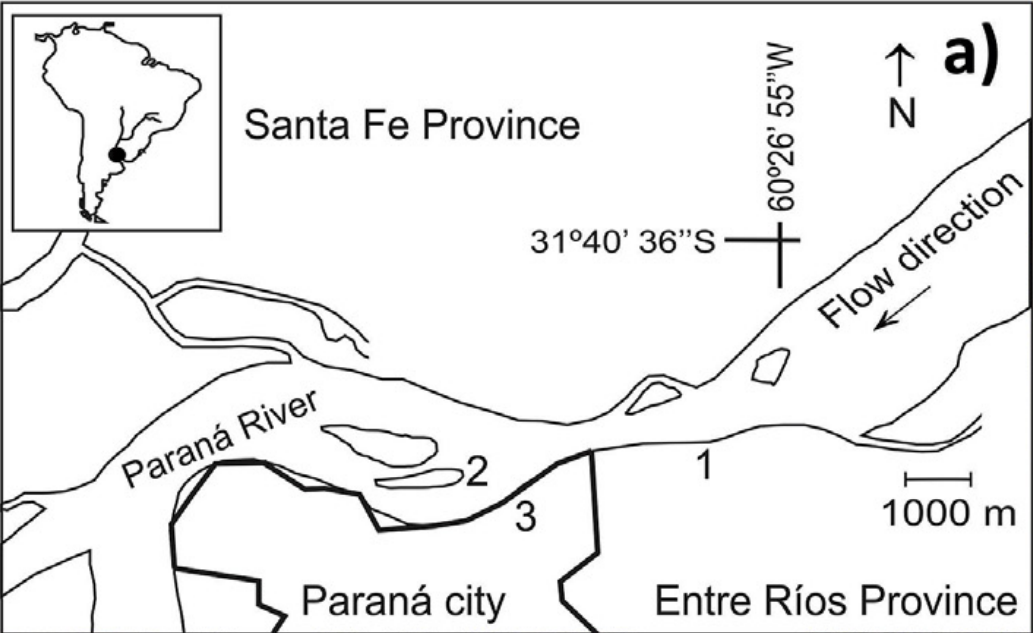
\includegraphics[width=\linewidth]{figura1/figura1a.png}
		\caption{En el Sur Global}
		\label{fig:sur_global}
	\end{subfigure}
	\begin{subfigure}[b]{0.45\linewidth}
		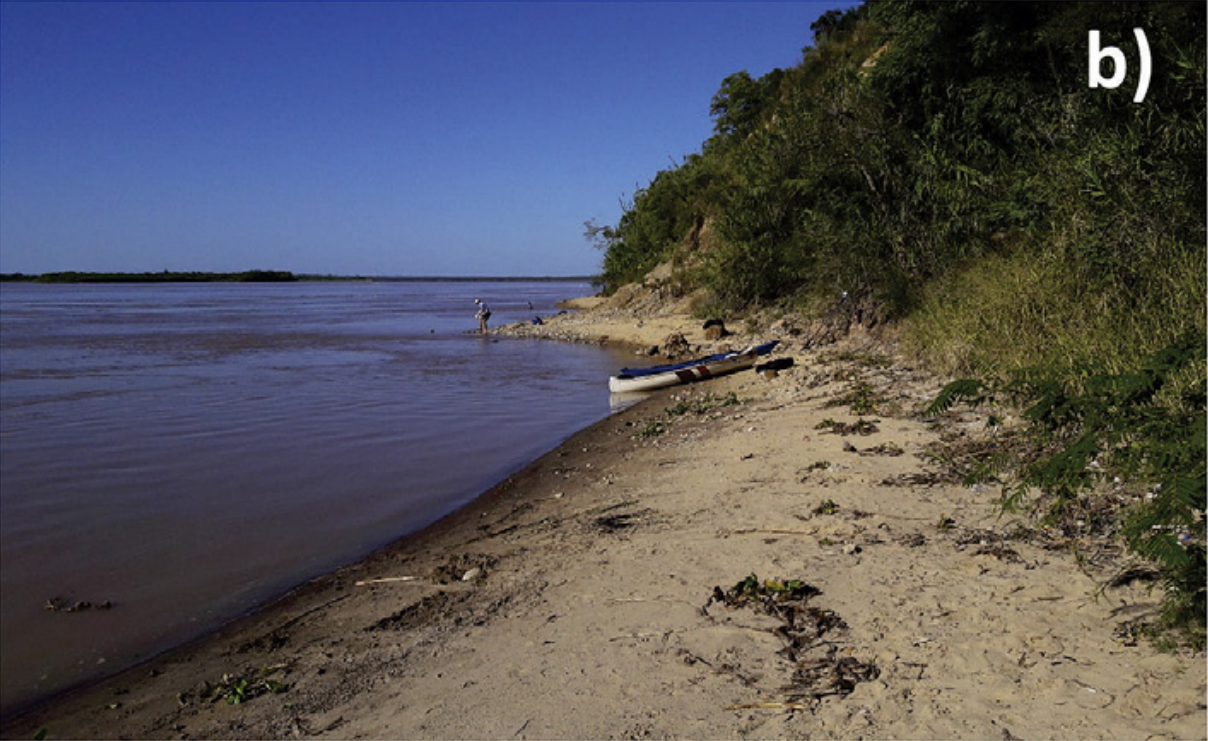
\includegraphics[width=\linewidth]{figura1/figura1b.png}
		\caption{Playa Escondida.}
		\label{fig:playa_escondida}
	\end{subfigure}
	\begin{subfigure}[b]{0.45\linewidth}
		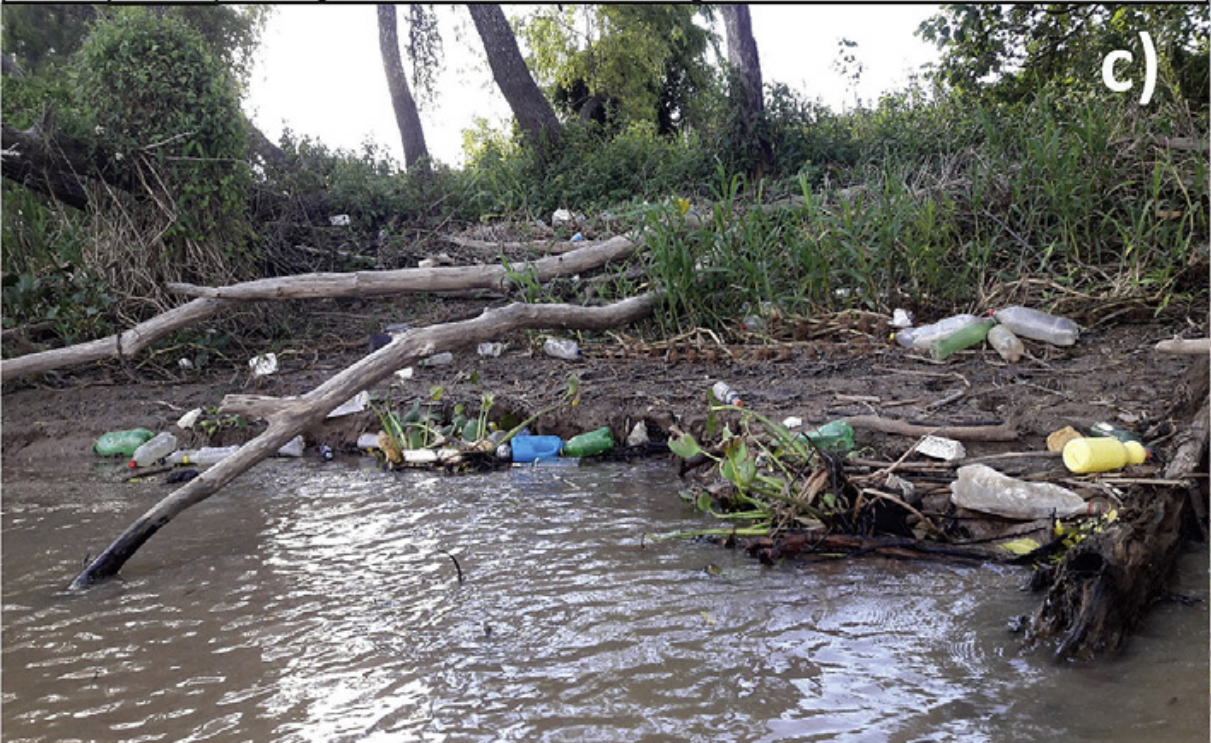
\includegraphics[width=\linewidth]{figura1/figura1c.png}
		\caption{Isla Curupí.}
		\label{fig:isla_curupi}
	\end{subfigure}
	\begin{subfigure}[b]{0.45\linewidth}
		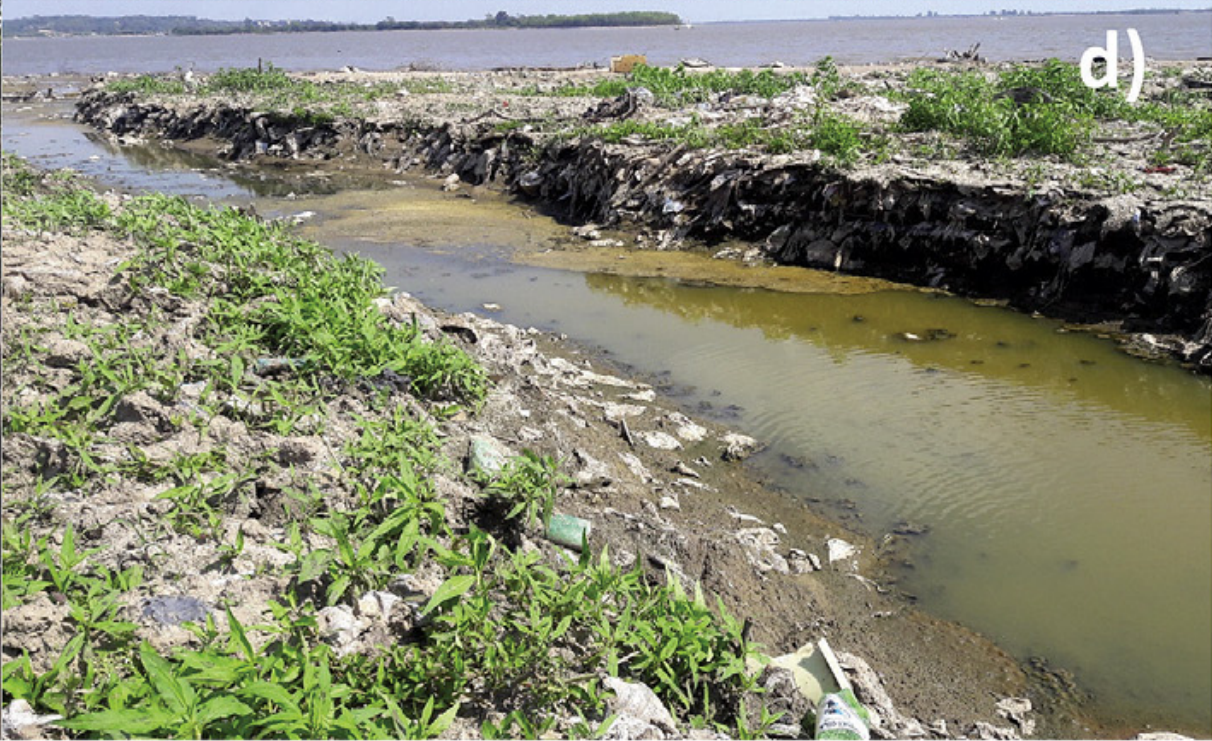
\includegraphics[width=\linewidth]{figura1/figura1d.png}
		\caption{\tiny Playa Thompson (en la confluencia del arroyo urbano Las Viejas con el canal principal de Paraná)}
		\label{fig:playa_thompson}
	\end{subfigure}
	\caption{Ubicación del río Paraná (área de estudio, provincia de Entre Ríos, Argentina)}
	\label{fig:ubicacion_rioParana}
	\vspace{-7mm}
\end{figure}

\textit{Prochilodus lineatus} (localmente llamado ``Sábalo'') es una especie de pez detritívoro dominante de gran importancia para la pesca comercial y artesanal \parencite{espinola2016response}. Para el análisis de peces, se obtuvieron 21 ejemplares frescos que fueron capturados con redes enmalle de $14$ y $16cm$ entre nudos opuestos en los respectivos sitios del área de estudio, respetando las políticas locales. Los peces se capturaron en las primeras horas de la mañana y se transportaron al laboratorio en hielo en 3 horas. Para cada individuo, se midió la longitud total ($cm$) y también se determinó el peso corporal total ($g$). Posteriormente, las muestras de pescado se abrieron con un bisturí y se retiraron los tractos gastrointestinales y se colocaron inmediatamente en cristalería limpia para minimizar el riesgo de contaminación del laboratorio \parencite{BESSA2018575}. Además de los métodos que se describen a continuación, también observamos el color de las partículas ingeridas para identificar las posibles preferencias.

Para evitar la contaminación por microplásticos, potencialmente presentes en el entorno del laboratorio, era obligatorio el uso de batas de laboratorio, guantes y mascarillas de algodón. Además, la cristalería y el lugar de trabajo se limpiaron con una solución de etanol ($96\%$) antes de comenzar todos los experimentos para conservar un ambiente estéril. Desde el inicio de las operaciones hasta la observación al microscopio, las muestras se cubrieron con papel de aluminio.

La materia orgánica presente en las muestras fue digerida con peróxido de hidrógeno ($H_2O_2$)($30\%$) a $60 ^{\circ}C$ (~\cite{PAZOS201785};~\cite{JABEEN2017141}). Según ~\cite{JABEEN2017141}, $H_2O_2$ es un agente oxidante que no cambia ni blanquea la estructura de las partículas microplásticas. De acuerdo con nuestros principios ambientales, todas las campañas de muestreo se realizaron en kayaks (emisión cero y contaminación acústica libre).

\subsection{Análisis y procesamiento de muestras}
Las partículas macroplásticas fueron lavadas, contadas y clasificadas en el laboratorio (ítem por ítem). La clasificación tuvo en cuenta su origen funcional (por ejemplo, envoltorios de alimentos, envases, botellas de bebidas, bolsas de la compra, productos de cuidado personal, etc.) siguiendo la NOAA \parencite{lippiatt2013marine} y la composición de la resina. Se utilizó el Sistema de Codificación de Identificación de Resinas de ASTM Internacional \parencite{RIC} para reconocer la resina plástica utilizada en los macroplásticos manufacturados \parencite{GASPERI2014163}. Como el procedimiento posterior no siempre fue posible de usar (en ocasiones este código se pierde o no es claramente visible), utilizamos un espectrofotómetro FTIR Shimadzu IR Prestige $21^{TM}$ para identificar la resina plástica \parencite{SONG2015202}.

Según ~\cite{GUNDOGDU2017341}, los mesoplásticos se contaron y clasificaron en: espuma de poliestireno, plástico duro, hilo de pescar y películas.

La separación de microplásticos se realizó siguiendo el método propuesto por~\cite{masura2015laboratory}. Por lo tanto, las muestras completas se secaron a $60 ^{\circ}C$ por $24 horas$, se pesaron y se tamizaron a través de un tamiz de acero inoxidable de $350mm$ de tamaño de malla utilizando un agitador de tamices Retsch $^{TM}$. El material restante se transfirió a un vaso de precipitados de $1 L$ para oxidación con peróxido húmedo al $30\%$ ($H_2O_2$) y se colocó en una placa caliente a $60 ^{\circ}C$ hasta que se digerió todo el material orgánico \parencite{T.Yonkos2014}. Una vez completado, se lavó $H_2O_2$ usando agua destilada a través de una malla de $350mm$. Posteriormente, se agregó una solución salina concentrada de $NaCl$ ($1.2 g cm^{-3}$) y se agitó fuertemente durante aproximadamente $1min$ \parencite{Hidalgo-Ruz2012}. Posteriormente, el sobrenadante con microplásticos flotantes se extrajo y se lavó con agua destilada para su posterior procesamiento. Este último paso se repitió tantas veces como fue necesario para atrapar cada partícula de plástico flotante.

Los microplásticos se separaron de otros materiales (presentes en el sobrenadante) y se clasificaron con un microscopio estereoscópico con zoom Boeco$^{tm}$ y un microscopio binocular Nikon$^{TM}$ ($10-40x$). Usamos los criterios sugeridos por~\cite{noren2007small} para identificar microplásticos. Sin embargo, los artículos de origen dudoso se analizaron con un espectrofotómetro FT--IR para confirmar (o rechazar) su composición plástica (~\cite{FRIAS201489};~\cite{LI2016177}). Los rangos de espectros se establecieron en $4000-400 cm^{-1}$, utilizando el software IRsolution Agent. Los espectros resultantes se compararon directamente con las bases de datos de la biblioteca de referencia.

Los microplásticos se clasificaron en espuma de poliestireno (marca registrada de espuma de poliestireno extruido de celda cerrada), plástico duro, película, fibra y rollo de fibra (fibras muy grandes retorcidas), según~\cite{doi:10.1139/cjfas-2014-0281} y ~\cite{GUNDOGDU2017341}.

\subsection{Análisis de datos}
Se crearon tablas y figuras para identificar la presencia, abundancia y tipo de desechos plásticos con el fin de comparar los sitios de muestreo entre sí. Se realizaron correlaciones entre los diferentes rangos de incautación de plástico. Con el fin de probar patrones espaciales de similitud en la abundancia y el tipo de microplásticos, se realizó un análisis canónico de coordenadas principales (CAP). El CAP es un análisis de ordenación restringido que calcula los ejes de coordenadas principales no restringidos seguidos de un análisis discriminante canónico en las coordenadas principales para maximizar la separación entre grupos predefinidos \parencite{anderson2004cap}. El índice de disimilitud de Bray-Curtis y 999 permutaciones fueron los parámetros seleccionados en este procedimiento. Se llevaron a cabo análisis de varianza multivariados permutacionales unidireccionales posteriores (PERMANOVA) \parencite{Anderson2001} para determinar las diferencias entre las puntuaciones del Eje 1 de CAP.

Los análisis estadísticos se realizaron utilizando el software CAP versión 1.0 \parencite{anderson2004cap} y el software MULTIV, versión 2.4.2 \parencite{pillar2006multiv}, con un nivel de significación estadística $p<0.05$.

\section{Resultados}
\label{sec:resultados}

\begin{table}[h!b]
	\centering
	\caption{\scriptsize Tipo (origen/uso), densidad por transecto ($150m^{2}$), desviación estándar, abundancia ($\%$) y composición de resina de los desechos macroplásticos (total y por sitio de muestreo). Donde, HDPE: polietileno de alta densidad; LDPE: polietileno de baja densidad; PP: polipropileno; PS: poliestireno; EPS: poliestireno expandido; PET: tereftalato de polietileno; Nylon: poliamida seca; PE: polietileno; PVC: cloruro de polivinilo.}
	\label{tab:macroplasticos}
	\begin{tabular}{l p{2cm} l l}
		\noalign{\hrule height 1pt}
		\scriptsize Tipo de escombros               & \scriptsize N$^{\circ}$ of items per transect ($150 m^{2}$) and Standard Deviation & \scriptsize $\%$  & \scriptsize Resin                \\  \noalign{\hrule height 1pt}
		\scriptsize Bag                             & \scriptsize 166.2$\pm$252.1                                                        & \scriptsize 48.75 & \scriptsize HDPE, LDPE           \\
		\scriptsize Foodwrapper                     & \scriptsize 68.3$\pm$110.1                                                         & \scriptsize 20.05 & \scriptsize PP, PS               \\
		\scriptsize Styrofoam                       & \scriptsize 35.5$\pm$61.5                                                          & \scriptsize 10.42 & \scriptsize EPS                  \\
		\scriptsize Beverage bottle                 & \scriptsize 30.7$\pm$31.2                                                          & \scriptsize 9.00  & \scriptsize PET                  \\
		\scriptsize Fishing line                    & \scriptsize 8.5$\pm$15.7                                                           & \scriptsize 2.49  & \scriptsize Nylon                \\
		\scriptsize Bottle cap                      & \scriptsize 4.7$\pm$6.3                                                            & \scriptsize 1.37  & \scriptsize PP                   \\
		\multicolumn{4}{ l }{\scriptsize (hard)}                                                                                                                                                \\
		\scriptsize Cleaning bottle                 & \scriptsize 3.2$\pm$4                                                              & \scriptsize 0.93  & \scriptsize HDPE, PET            \\
		\scriptsize Sanitary napkin                 & \scriptsize 1.7$\pm$4.1                                                            & \scriptsize 0.49  & \scriptsize PP, PE               \\
		\scriptsize Household                       & \scriptsize 1$\pm$0.4                                                              & \scriptsize 0.29  & \scriptsize Undetermined         \\
		\multicolumn{4}{ l }{\scriptsize appliances}                                                                                                                                            \\
		\scriptsize Personal care                   & \scriptsize 0.8$\pm$2                                                              & \scriptsize 0.24  & \scriptsize PP, HDPE, PET, PDPE, \\
		\multicolumn{2}{ l }{\scriptsize container} & \multicolumn{2}{ r }{\scriptsize Varies}                                                                                                  \\
		\scriptsize Strapping band                  & \scriptsize 0.8$\pm$2                                                              & \scriptsize 0.24  & \scriptsize Polyester, PP        \\
		\scriptsize Cloth                           & \scriptsize 0.3$\pm$0.5                                                            & \scriptsize 0.10  & \scriptsize Polyester            \\
		\scriptsize Bottle label                    & \scriptsize 0.2$\pm$0.4                                                            & \scriptsize 0.05  & \scriptsize PET, PP, PVC         \\
		\scriptsize Straw                           & \scriptsize 0.2$\pm$0.4                                                            & \scriptsize 0.05  & \scriptsize PP                   \\
		\scriptsize Diaper                          & \scriptsize 0.2$\pm$0.4                                                            & \scriptsize 0.05  & \scriptsize PP, PET              \\
		\scriptsize Cigarette butt                  & \scriptsize 0.2$\pm$0.4                                                            & \scriptsize 0.05  & \scriptsize Cellulose acetate    \\
		\scriptsize Others                          & \scriptsize 15.2$\pm$19.2                                                          & \scriptsize 4.45  & \scriptsize Undetermined         \\
		\scriptsize Total                           & \scriptsize 340.8                                                                  & \scriptsize 100   & \scriptsize                      \\ \hline
		\multicolumn{4}{ l }{\scriptsize \textbf{Site}}                                                                                                                                         \\ \noalign{\hrule height 1pt}
		\scriptsize \textbf{Escondida}              & \scriptsize 52$\pm$42.4                                                            & \scriptsize 5.1   & \scriptsize                      \\
		\scriptsize \textbf{Curupí}                 & \scriptsize 190$\pm$77.1                                                           & \scriptsize 18.6  & \scriptsize                      \\
		\scriptsize \textbf{Thompson}               & \scriptsize 780$\pm$14.1                                                           & \scriptsize 76.3  & \scriptsize                      \\ \noalign{\hrule height 1pt}
	\end{tabular}
\end{table}

\subsection{Macroplásticos}
Registramos un total de 18 categorías de desechos macroplásticos (según la clasificación de la NOAA;~\cite{lippiatt2013marine}); siendo bolsa, envoltorio de alimentos, poliestireno y botella de bebida las partículas más abundantes, representando casi el $80\%$ del total (Tabla \ref{tab:macroplasticos}).

Los tres sitos de muestreo tiene fuertes diferencias en la cantidad (número de elementos) y el tipo de desechos macroplásticos (Fig. \ref{fig:macro}). Así, la playa Escondida ($4 km$ aguas arriba de la ciudad de Paraná) mostró los valores más bajos (52 macro-ítems por transecto; $150 m^{2}$), con una composición heterogénea de tipos de plástico (13 categorías diferentes) pero dominada por líneas de pesca (23 ítems). La isla Curupí (frente a la ciudad de Paraná), estuvo dominada por solo 2 tipos de macroplásticos: botellas de bebidas (81) y fragmentos de poliestireno (99). Finalmente, la playa de Thompson (ligeramente aguas abajo del outlet de Las Viejas) mostró un claro predominio de bolsas de compras (490; muchos colores y texturas diferentes) y envoltorios de alimentos (202.5), teniendo la mayor cantidad de plásticos: 757.5 artículos por transecto (es decir $5.05$ partículas macroplásticas por $m^{2}$), 14 veces más que la playa Escondida. De lejos, las resinas plásticas más abundantes fueron HDPE, LDPE, PP y PS en la playa Thompson, EPS y PET en la isla Curupí y Nylon en al playa Escondida. Se encontraron resinas de acetato de celulosa, poliéster y PVC a bajas densidades.

\begin{table}[h!t]
	\centering
	\caption{\scriptsize Tipo, densidad ($m^{2}$), derivación estándar, y abundancia ($\%$) de detritos mesoplásticos por sitio de muestreo.}
	\label{tab:mesoplasticos}
	\begin{tabular}{ p{1.2cm} l l l p{1cm} l }
		\noalign{\hrule height 1pt}
		\scriptsize Mesoplastic Type & \scriptsize Escondida & \scriptsize Curupí & \scriptsize Thompson & \scriptsize Standard deviation & \scriptsize $\%$ \\ \noalign{\hrule height 1pt}
		\scriptsize Styrofoam        & \scriptsize 47.8      & \scriptsize 35.5   & \scriptsize 16       & \scriptsize 48.3               & \scriptsize 89.3 \\
		\scriptsize Hard plastics    & \scriptsize 7.5       & \scriptsize 0      & \scriptsize 2.5      & \scriptsize 7.6                & \scriptsize 10   \\
		\scriptsize Fishing tape     & \scriptsize 0.2       & \scriptsize 0      & \scriptsize 0        & \scriptsize 0.2                & \scriptsize 0.2  \\
		\scriptsize Cassette tape    & \scriptsize 0.2       & \scriptsize 0      & \scriptsize 0        & \scriptsize 0.2                & \scriptsize 0.2  \\
		\noalign{\hrule height 1pt}
		\scriptsize Total (mean)     & \scriptsize 55.6      & \scriptsize 35.5   & \scriptsize 18.5     & \scriptsize 18.6               & \scriptsize 100  \\ \noalign{\hrule height 1pt}
	\end{tabular}
\end{table}

\subsection{Mesoplásticos}
A diferencia de los macroplásticos, los mesoplásticos tuvieron la mayor abundancia den la playa Escondida (55.6 ítems $m^{-2}$), seguida de la isla Curupí (35.5 ítems $m^{-2}$) y la playa Thompson (solo 18.5 partículas por $m^{2}$; Fig. \ref{fig:meso}). La abundancia promedio de mesoplástico estuvo cerca de 46 ítems $m^{-2}$, siendo el plástico espumado (Styrofoam) la categoría dominante (41.1 ítems $m^{-2}$) (Tabla \ref{tab:mesoplasticos}).

\begin{figure}[h!t]
	\centering
	\begin{subfigure}[b]{0.3\linewidth}
		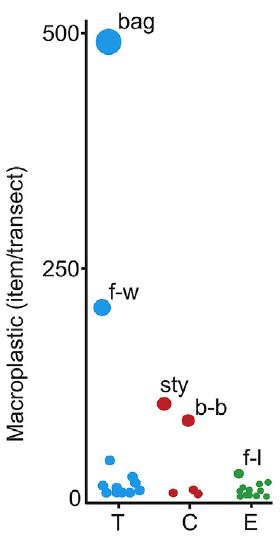
\includegraphics[width=\linewidth]{figura2/figura2a.png}
		\caption{macro-}
		\label{fig:macro}
	\end{subfigure}
	\begin{subfigure}[b]{0.3\linewidth}
		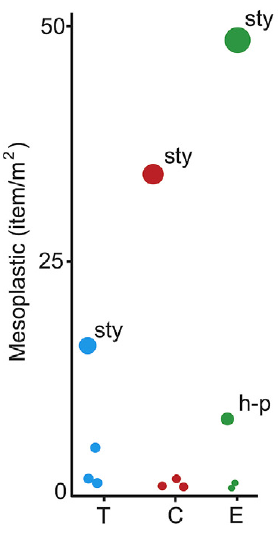
\includegraphics[width=\linewidth]{figura2/figura2b.png}
		\caption{meso-}
		\label{fig:meso}
	\end{subfigure}
	\begin{subfigure}[b]{0.3\linewidth}
		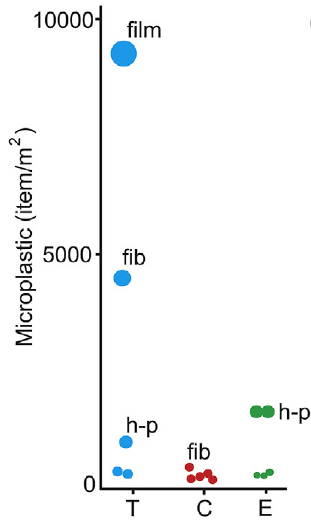
\includegraphics[width=\linewidth]{figura2/figura2c.png}
		\caption{microplástico}
		\label{fig:micro}
	\end{subfigure}
	\caption{Gráfico de burbujas que muestra las densidades en cada área de muestreo. Donde: f-w: envoltura de alimentos, pocilga: espuma de poliestireno, b-b: botella de bebida, hilo de pescar, h-p: pieza de plástico duro, fib: fibra.}
	\label{fig:densidades}
\end{figure}

\begin{table}[h!b]
	\centering
	\caption{\scriptsize Tipo, densidad ($m^{2}$), derivación estándar, y abundancia ($\%$) de detritos microplásticos por sitio de muestreo.}
	\label{tab:microplasticos}
	\begin{tabular}{ l l l l l l l }
		\noalign{\hrule height 1pt}
		\tiny               & \tiny Escondida & \tiny Curupí & \tiny Thompson & \tiny Standard deviation & \tiny $\%$ & \tiny Category  \\\hline
		\tiny Fiber         & \tiny 1431.4    & \tiny 90     & \tiny 4466.9   & \tiny 1899.6             & \tiny 33.1 & \tiny Primary   \\
		\tiny Hard plastics & \tiny 1424.2    & \tiny 18.8   & \tiny 421.7    & \tiny 51.8               & \tiny 0.9  & \tiny Secondary \\
		\tiny Styrofoam     & \tiny 33.2      & \tiny 11.3   & \tiny 36.2     & \tiny 2645.4             & \tiny 17.5 & \tiny Secondary \\
		\tiny Film          & \tiny 0         & \tiny 0.8    & \tiny 8953.5   & \tiny 6772.3             & \tiny 48.2 & \tiny Secondary \\
		\tiny Fiber-roll    & \tiny 0         & \tiny 0      & \tiny 72.9     & \tiny 54.5               & \tiny 0.4  & \tiny Primary   \\
		\noalign{\hrule height 1pt}
		\tiny Total (mean)  & \tiny 2899      & \tiny 131    & \tiny 12687    & \tiny 8548.1             & \tiny 100  & \tiny           \\ \noalign{\hrule height 1pt}
	\end{tabular}
\end{table}

\subsection{Microplásticos}
Las películas y fibras fueron los elementos dominantes en las muestras de microplásticos (Tabla \ref{tab:microplasticos}). Se encontró un promedio de 4654 fragmentos de microplásticos (por $m^{2}$) en los sedimentos de la costa de los tres muestreos (playas e islas). En la playa Thompson se registró un promedio de 12687 micropartículas $m^{-2}$  ($81\%$ del total), pero solo 131 en la isla Curupí (Fig. \ref{fig:micro}). La película y la fibra de microplástico eran extremadamente abundantes en la playa de Thompson.

El CAP (y el subsiguiente PERMANOVA) mostró diferencias significativas en la abundancia y el tipo de microplásticos entre las tres playas (sitios de muestreo)($p-valores=<0.003$; Suma de cuadrados (Q) dentro de los grupos $=2.829$)(Fig. \ref{fig:cap}).

La Tabla \ref{tab:correlaciones} muestra que los valores de densidad de las clases de tamaño (macro, meso y microplástico) no fueron sustitutos entre sí (no se detectaron correlaciones). Si bien se pudieron detectar algunas tendencias débiles (ej.: valores de alta concentración de macro y microplásticos en la playa de Thompson), no fueron estadísticamente significativas. Particularmente, la abundancia mesoplástica mostró una tendencia completamente independiente. Por ejemplo: los valores más bajos de macroplástico se encontraron en la playa Escondida, pero el mesoplástico mostró la mayor concentración en la misma playa. Mientras que las concentraciones más altas de macro y microplásticos se encontraron en la playa de Thompson, la concentración de mesoplástico fue la más baja.

\begin{table}[h!t]
	\centering
	\caption{\scriptsize Correlaciones entre los diferentes rangos de incautación de plástico.}
	\label{tab:correlaciones}
	\begin{tabular}{ p{4cm} p{2cm} l }
		\noalign{\hrule height 1pt}
		\scriptsize                      & \scriptsize $r^{2}$ & \scriptsize $p-value$ \\ \noalign{\hrule height 1pt}
		\scriptsize Macro- $vs.$ meso-p  & \scriptsize 0.006   & \scriptsize 0.85      \\
		\scriptsize Meso- $vs.$ micro-p  & \scriptsize 0.022   & \scriptsize 0.72      \\
		\scriptsize Micro- $vs.$ macro-p & \scriptsize 0.199   & \scriptsize 0.27      \\
		\noalign{\hrule height 1pt}
	\end{tabular}
\end{table}

\subsection{Ingestión de pescado}
Todos los peces estaban contaminados con al menos un microplástico. El número de elementos registrados en el tracto digestivo de \textit{P. lineatus} adulto promedió $9.9$ partículas microplásticas. El valor máximo de partículas microplásticas registradas en un individuo fue 27 (Fig \ref{fig:particulas_microplasticas}). Los tamaños de las partículas oscilaron entre $0.5$ y $3mm$ y los colores registrados fueron azul (la mayoría), negro, amarillo, rojo y transparente.

\begin{figure}[h!b]
	\centering
	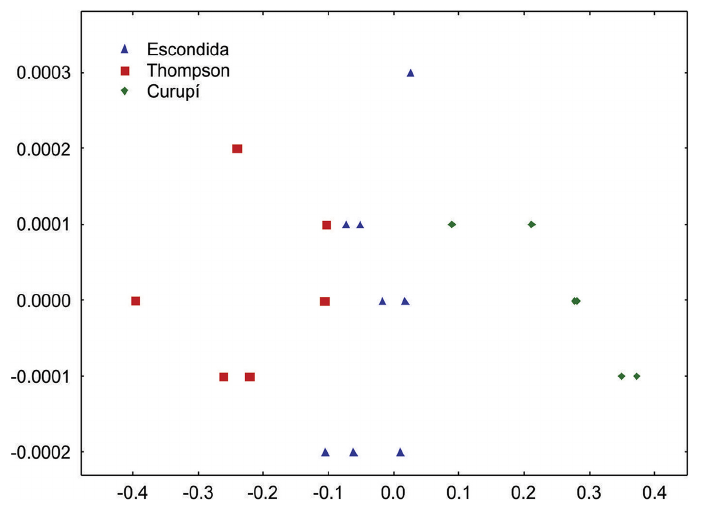
\includegraphics[width=0.5\textwidth]{figura3.png}
	\caption{Gráfica de ordenación del Análisis Canónico de Coordenadas Principales (CAP) que muestra diferencias significativas en abundancia y tipo de microplásticos entre los tres sitios de muestreo (playa Escondida, playa Thompson, isla Curupí).}
	\label{fig:cap}
\end{figure}

\begin{figure}[h!t]
	\centering
	\begin{subfigure}[b]{0.6\linewidth}
		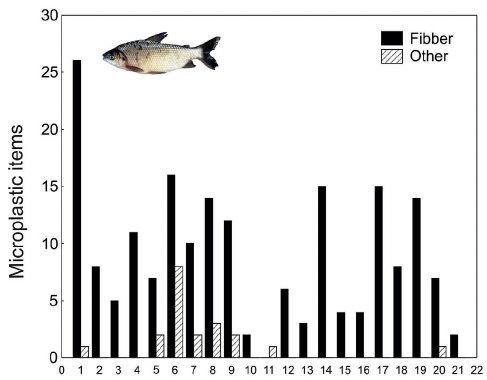
\includegraphics[width=\linewidth]{figura4/figura4a.png}
		\caption{Número de artículos}
		\label{fig:numero_articulos}
	\end{subfigure}
	\begin{subfigure}[b]{0.2\linewidth}
		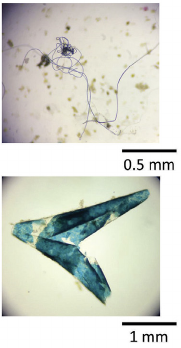
\includegraphics[width=\linewidth]{figura4/figura4b.png}
		\caption{Fibras y un trozo de película plástica}
		\label{fig:fibra_pelicula}
	\end{subfigure}
	\caption{Partículas microplásticas (fibras y otras) encontradas en el tracto digestivo de P. Lineatus.}
	\label{fig:particulas_microplasticas}
\end{figure}

\section{Discusiones}
\label{sec:discusiones}

\subsection{Concentraciones masivas de plástico: cuestiones geopolíticas y sociales}%
Los materiales macroplásticos son la forma más visible de contaminación plástica.~\cite{Blettler2017} reportaron un promedio de 172.5 ítems macroplásticos por transecto de $150 m^{2}$ ($\sim 1.15$ ítems $m^{2}$) en un lago de llanura aluvial del río Paraná, ubicado a solo 18 km de nuestra área de muestreo. En el presente estudio, encontramos casi el doble de esa cantidad: $340.8$ macroplásticos por $150 m^{2}$ ($\sim 2.27 m^{2}$).

Si bien se han realizado varios estudios sobre macroplásticos en la superficie del agua de ríos (~\cite{GASPERI2014163};~\cite{faure2015};~\cite{Baldwin2016};~\cite{LAHENS2018661}) y lagos \parencite{faure2015}, los estudios macroplásticos en sedimentos fluviales aún son escasos, especialmente para las playas. Algunos ejemplos incluyen~\cite{imhof2013contamination} en el lago de Garda (Italia) y~\cite{faure2015}en 6 lagos de Suiza. Sin embargo, la comparación directa con el presente estudio es inviable ya que estos autores consideraron macroplásticos como partículas superiores a $5 mm$ (incluido el tamaño mesoplástico).

La gran cantidad de detritos macroplásticos registrados en la playa Thompson e isla Curupí, así como el origen de los mismos (residuos domiciliarios, Tabla \ref{tab:macroplasticos}), sugieren un deficiente procesamiento de recolección y disposición final d residuos en la ciudad de Paraná. La gestión de residuos es uno de los problemas ambientales clave relacionados con los hidrosistemas urbanos a escala global, sin embargo, en el Sur Global todavía se basa fuertemente en el vertido incontrolado y/o la basura \parencite{GUERRERO2013220}. Como resultado, ocurren serios problemas ambientales \parencite{ALKHATIB20101131} y una creciente contaminación plástica \parencite{Battulga2019}, particularmente en los sistemas de agua dulce. Los municipios de los países de bajos ingresos están gastando una proporción menor de sus presupuestos en la gestión de desechos y, sin embargo, más del $90\%$  de los desechos en los países de bajos ingresos todavía se arrojan abiertamente \parencite{Kaza2018}. Además, el aumento de la población y el aumento de los niveles de consumo han acelerado enormemente la tasa de generación de residuos sólidos en Argentina (tasas de generación de residuos: $1.14 kg$ / cápita / día;~\cite{Kaza2018}). El presente estudio muestra, en parte, esta tendencia global.

La mayoría de los macroplásticos registrados en la presente investigación fueron bolsas de la compra, seguidos de envoltorios de alimentos y envases de espuma (casi el $80\%$; Tabla \ref{tab:macroplasticos}). Las primeras comunidades en adoptar la norma de las bolsas antiplásticas fueron las del Sur Global, mientras que las del Norte Global lo hicieron mucho más recientemente \parencite{Clapp2009}. Sin embargo, no se adoptó una ordenanza municipal contra las bolsas de plástico en la ciudad de Paraná antes de 2017.

Los resultados de los estudios de microplásticos disponibles en sistemas de agua dulce son extremadamente variables de acuerdo con la metodología utilizada (por ejemplo, $m^{2}$, $m^{3}$, $l$, $kg$), medio ambiente (río, lago, embalse, estuario, alcantarillado, etc.), y compartimento de muestreo (superficie o columna de agua, sedimento del fondo o de la playa, etc.). Como resultado, las comparaciones entre estudios mundiales son muy difíciles. Encontramos un promedio de 5239 microplásticos $m^{2}$ (rango de tamaño: $0.35-5 mm$) en los sedimentos del banco del río Paraná, que van desde solo 75 hasta un máximo de $34443$ microplásticos $m^{2}$ (Tabla \ref{tab:microplasticos}).~\cite{doi:10.1139/cjfas-2014-0281} encontraron alrededor de 13832 $m^{2}$ de microperlas de polietileno, retenidas por un tamiz de $0.5mm$, de efluentes industriales en los sedimentos del río San Lorenzo (Canadá).~\cite{Klein2015} tiene un registro de aproximadamente 228-3763 micropartículas $kg^{-1}$ en los sedimentos costeros de los ríos Rin y Main en Alemania (tamaño microplástico: $0.2-5mm$). Además,~\cite{SU2016711}han informado de un rango de $15-1600$ microplásticos $l^{-1}$ ($>0.3 mm$) en el río Yangtze medio-bajo (China),~\cite{WANG20171369} registraron $178-544$ microplásticos $l^{-1}$ ($<5 mm$) en los sedimentos de río Beijiang, y~\cite{PENG2017283} encontraron $410-1600$ microplásticos $kg^{-1}$ ($0.05-5 mm$) en algunos ríos de Shaghai, la mayoría de los fragmentos de dobladillo, esferas y fibras.

~\cite{Blettler2017}, utilizando la misma metodología que el presente estudio, han registrado un promedio mucho más bajo de $704$ microplásticos $m^{-2}$ (rango de tamaño: $0.35-5mm$) en sedimentos de playa de ambientes lénticos del río Paraná (un lago de llanura aluvial ubicado a $18 km$ de distancia del área de muestreo del presente estudio).~\cite{XIONG2018899} reportaron $50-1292$ microplásticos $m^{-2}$ ($>0.1mm$) en el lago Qinghai (China); la mayoría eran películas, fibras y espumas.

A pesar de las limitaciones y debilidades de las comparaciones anteriores (es decir, diferentes rangos de tamaño, unidades, ambientes), la información disponible sugiere una contaminación microplástica significativa presente en los sedimentos del río Paraná.

La variación de la abundancia y el tipo de microplásticos entre los sitios de muestreo fue estadísticamente significativa (Fig. \ref{fig:particulas_microplasticas}), mostrando una clara diferenciación por playa de muestreo. La playa de Thompson mostró la mayor concentración de microplásticos, mientras que Escondida reveló la distribución más heterogénea (las estaciones de muestreo variaron de baja a alta concentración de microplásticos).

El microplástico puede presentarse en forma primaria (perlas) o secundaria (originada por la descomposición de artículos plásticos más grandes;~\cite{COLE20112588}). Aún se desconoce la importancia relativa de las fuentes primarias y secundarias de microplásticos. Encontramos ambos, pero los secundarios fueron considerablemente más abundantes (Tabla \ref{tab:microplasticos})

Se debe prestar especial atención a la ropa sintética, que es una fuente importante de fibras a través del lavado \parencite{Conkle2018}. En nuestro estudio, la fibra fue el único microplástico primario registrado \parencite{Cole2013}. Sin embargo, cabe señalar que algunos autores consideran la fibra como secundaria (por ejemplo:~\cite{dris2015microplastic}). Otros microplásticos primarios como microperlas, cápsulas o gránulos (utilizados en cosméticos y productos de cuidado personal, depuradores industriales utilizados para limpieza con chorro abrasivo y gránulos vírgenes utilizados en procesos de fabricación de plástico, respectivamente) estaban ausentes. Se observó una falta similar de microperlas en el río Yangtze \parencite{ZHANG2015117} y el embalse de las Tres Gargantas \parencite{Zhang2017} en China, el río Saigón en Vietnam \parencite{LAHENS2018661} y el Estuario del río Paraná en Argentina \parencite{PAZOS2018134}. No obstante, se observó una gran presencia de microperlas en los ríos Rin y San Lorenzo (~\cite{Mani2015} y~\cite{doi:10.1139/cjfas-2014-0281}, respectivamente) y en los grandes Lagos Laurentinos \parencite{ERIKSEN2013177}. En algunos países que se benefician de instalaciones avanzadas de tratamiento de residuos (principalmente en Europa y América del Norte), las emisiones de microplásticos secundarios son incluso más bajas que las de los microplásticos primarios \parencite{gouin2015}. Las pérdidas de microplásticos primarios pueden ocurrir durante las etapas de producción, transporte o reciclaje de plásticos, o durante la fase de uso de productos que contienen microplásticos (por ejemplo, microperlas originadas de limpiadores faciales ampliamente utilizados en países desarrollados;~\cite{NAPPER2015178};~\cite{gouin2015}). Esto contrasta con los microplásticos secundarios que se originan principalmente a partir de residuos mal gestionados durante la eliminación de productos que contienen plásticos \parencite{Boucher2017}. La ausencia de microperlas en el sistema del río Paraná podría explicarse por estas diferencias en los hábitos de consumo y la gestión de residuos entre sociedades y países. Aquí, casi el $50\%$ de los microplásticos registrados fueron partículas de película (como producto secundario del proceso avanzado de descomposición de bolsas), $33.1\%$ de fibras (utilizadas en textiles) y $18.7\%$ resultantes de partículas más grandes de plástico de origen incierto que se descomponen en elementos más pequeños (probablemente botella de bebida, envoltorio de comida y espumas)(Tabla \ref{tab:microplasticos}). Por el contrario, otros estudios en ríos de países en desarrollo han informado de un predominio de fibras microplásticas (~\cite{ZHANG2015117};~\cite{LAHENS2018661}), incluso en el estuario del río Paraná \parencite{PAZOS2018134}.

Las proporciones variables entre macro o mesoplásticos en nuestro estudio han demostrado que estos datos no pueden servir como sustitutos para el monitoreo de microplásticos (Tabla \ref{tab:correlaciones}). Esto es importante ya que los voluntarios pueden realizar fácilmente estudios de desechos de macroplásticos, que han desempeñado un papel importante en muchos programas de monitoreo de desechos \parencite{RIBIC2012994}.

\subsection{Papel de las corrientes urbanas en la difusión del plástico}

Los ríos y arroyos urbanos sufren de múltiples factores estresantes interactivos, especialmente en el Sur Global (~\cite{WANG20171369};~\cite{wantzen2019urban}). En este estudio, el arroyo urbano Las Viejas parece jugar un papel crucial transportando grandes cantidades de residuos plásticos y depositándolos en la playa Thompson, inmediatamente aguas abajo hasta la confluencia con el río Paraná (Fig. \ref{fig:playa_thompson}). Esta área de muestreo mostró la mayor concentración de desechos macro y microplásticos (Figs. \ref{fig:densidades} y \ref{fig:particulas_microplasticas}). El arroyo Las Viejas discurre por toda la ciudad de Paraná, concentrando y transportando los residuos sólidos municipales mal gestionados. Según~\cite{Xu2019} el desarrollo de sistemas de alcantarillado no ha alcanzado la velocidad de urbanización en los países en desarrollo, con graves consecuencias para la calidad del agua de los ríos urbanos. Por lo tanto, muchos ríos urbanos se convierten en los puntos finales de la contaminación plástica (\cite{McCormick2014};~\cite{Mccormick2016}). De la misma manera que las lluvias y las inundaciones severas pueden aumentar drásticamente los niveles de plástico en el mar \parencite{GUNDOGDU2018342}, es muy probable que el mismo fenómeno opere en arroyos urbanos que descargan en grandes sistemas fluviales.

Por otro lado, la isla Curupí presentó un promedio de 190 macroplásticos por transecto (contra 780 en el Thompson y solo 52 en la playa escondida; Tabla \ref{tab:macroplasticos}). Este sitio de muestreo estuvo dominado por dos artículos domésticos: botellas de bebidas y fragmentos de empaque de espuma (espuma de poliestireno; Fig. \ref{fig:densidades}). Suponemos que estos plásticos legaron del arroyo Las Viejas. Los desechos flotantes son transportados por la corriente de río Paraná y los vientos dominantes del sur hasta las costas de la isla Curupí. Este proceso podría verse facilitado por la alta flotabilidad de estos elementos (densidad del EPS: $11-32 kg m^{-3}$; mientras que la densidad del PET es de $950 kg m^{-3}$, las botellas inicialmente flotan debido al aire atrapado en el costado). De lo contrario, no se registraron bolsas de la compra y envoltorios de alimentos (artículos más abundantes en la playa Thompson) en la isla, lo que probablemente esté relacionado con su baja flotabilidad (densidad de HDPE: $950 kg m^{-3}$; LDPE: $917-930 kg m^{-3}$; PP: $946 kg m^{-3}$; PS: $1066 kg m^{-3}$).

Finalmente, no existe confluencias de ríos urbanos en la playa Escondida, que fue el área de muestreo menos contaminada. Esta playa mostró una composición de desechos plásticos completamente diferentes. Si bien las bolsas de la compra, la espuma de poliestireno y las botellas de bebidas estaban presentes, el artículo dominante era el hilo de pescar. Sugiere que el principal impacto lo dan los usuarios de la playa, la mayoría pescaderos artesanales y deportivos, y no los residuos municipales mal tratados provenientes de las grandes ciudades río arriba.

Los polímeros plásticos más comunes registrados en este estudio fueron HDPE, LPDE PP, PS Y EPS, que pueden ser muy dañinos para la fauna silvestre \parencite{Kyaw2012}. Además, el PP y el PS se han registrado ampliamente en las partículas de envoltorios de alimentos (Tabla \ref{tab:macroplasticos}). Finalmente, los productos de EPS (a menudo denominados Styrofoam$^{TM}$)(recipientes para llevar, vasos desechables, bandejas de espuma, etc.) se encontraron ampliamente en nuestro estudio (Tabla \ref{tab:macroplasticos}). El EPS se informa comúnmente como uno de los principales elementos de escombros recuperados de costas y playas en todo el mundo (~\cite{LEE2013349};~\cite{ocean}). Como resultado, los productos EPS ahora se discuten para prohibirlos en varios países (UNEP 2018). En el presente estudio, el EPS fue el detrito mesoplástico más abundante (casi el $90\%$; Tabla \ref{tab:mesoplasticos}).~\cite{ZBYSZEWSKI2014288} reportaron una proporción similar en mesoplásticos de los Grandes Lagos.

\subsection{Ingestión de plástico por pescado y posibles impactos}

Un estudio reciente reveló que se ha reportado ingestión de plástico en 427 especies de peces de más de 20 países alrededor del mundo \parencite{Azevedo-Santos2019}, causando bloqueos internos y lesiones en el tracto digestivo de los peces (~\cite{CANNON2016286};~\cite{NADAL2016517}). Registramos microplásticos en el tracto digestivo de $100\%$ de las muestras de \textit{P. lineatus} muestreadas, corroborando un estudio similar en el estuario de río Paraná \parencite{PAZOS201785}). Esto último podría explicarse por la estrategia de alimentación detritívora de esta especie y la gran cantidad de microplásticos registrados en el área de estudio. Por lo tanto, la frecuencia de aparición de microplásticos en peces del río Paraná parece ser más alta que en otros ríos de América del Sur. Por ejemplo, en el estuario del Amazonas y la costa norte de Brasil se encontraron microplásticos en el $13.8\%$ de los tractos digestivos examinados \parencite{Pegado2018}, el $23\%$ y el $13.4\%$ en el estuario de Goiana (\cite{POSSATTO20111098};~\cite{Ramos2012}, respectivamente). Sin embargo, reconocemos que el bajo número de ejemplares aquí estudiados no permite generalizaciones.

En nuestro estudio, la mayoría de los microplásticos registrados en el pescado fueron fibras ($90\%$). De acuerdo, varios estudios a nivel mundial también han reportado mayor número de fibras ingeridas en comparación con otros tipos de microplásticos (\cite{NEVES2015119};~\cite{BELLAS201655};~\cite{NADAL2016517};~\cite{PAZOS201785}). El razonamiento detrás del predominio de las fibras es la naturaleza diversa de este tipo de microplásticos, que puede tener su origen en la degradación de prendas de vestir, muebles y artes de pesca. De hecho, lavar (a través de una lavadora) una sola prenda sintética resultó en la liberación de aproximadamente 2000 microfibras (\cite{AnthonyBrowne2011};~\cite{CarneyAlmroth}). Los mesoplásticos ingeridos por los peces no se registraron en este estudio. De hecho, este tamaño de rango apenas se ha registrado en el tracto digestivo de los peces \parencite{JABEEN2017141}.

\section{Conclusiones}%
\label{sec:conclusiones}

\begin{enumerate}
	\item \item La concentración de desechos plásticos registrada (macro, meso y microplásticos) fue varias veces mayor que los valores reportados anteriormente en la llanura aluvial del río Paraná. Las comparaciones con otros estudios en todo el mundo siguen siendo difíciles, ya que los protocolos metodológicos aún no están estandarizados; sin embargo, sugieren niveles masivos de contaminación en este mega-río de América del Sur.
	\item Los macroplásticos registrados aquí tienen un origen doméstico (bolsas de compras, envoltorios de alimentos, botellas de bebidas y fragmentos de espuma de empaque), lo que sugiere una inadecuada recolección, procesamiento y disposición final de residuos en la región, que lamentablemente es recurrente en el Sur Global. La investigación adicional no debe pasar por alto los macroplásticos en esta región geopolítica, particularmente si se pretenden estimaciones confiables de los desechos plásticos globales que ingresan al océano desde los ríos.
	\item Los microplásticos secundarios (originados por la descomposición de artículos plásticos más grandes) eran más abundantes que los primarios (fabricados como microperlas, cápsulas, gránulos utilizados en la industria). Las microperlas (que se encuentran comúnmente en las regiones industrializadas) estaban ausentes en el río Paraná. Este hallazgo contrasta con estudios realizados en ambientes de agua dulce de países desarrollados, que sugieren una diferencia en los hábitos de consumo y los niveles de industrialización entre sociedades y economías del mundo desarrollado y en desarrollo.
	\item La mayoría de los desechos plásticos registrados proceden de un arroyo urbano altamente contaminando, que atraviesa la ciudad de Paraná. Los ríos urbanos, particularmente es el Sur Global, son vulnerables a diferentes procesos y actividades urbanas que provocan la contaminación y degradación del ecosistema hídrico.
	\item Registramos partículas microplásticas en el tracto digestivo del $100\%$ de los especímenes de \textit{P. lineatus}, la mayoría de ellas fibras. Si bien reconocemos el bajo número de peces recolectados, este hallazgo evidenció que los microplásticos han penetrado en las redes alimentarias acuáticas y nichos ecológicos en el río Paraná, lo que refuerza la necesidad de más estudios.
	      Contrariamente a nuestras expectativas, los elementos macroplásticos o mesoplásticos no servirían como sustitutos para los estudios de microplásticos (y viceversa), lo que sugiere que todos los tamaños de desechos plásticos deben considerarse en estudios posteriores.
\end{enumerate}

%
%
%
\printbibliography[title={Bibliografía}]
\end{document}
